% Created by tikzDevice version 0.12.6 on 2024-06-02 21:53:08
% !TEX encoding = UTF-8 Unicode
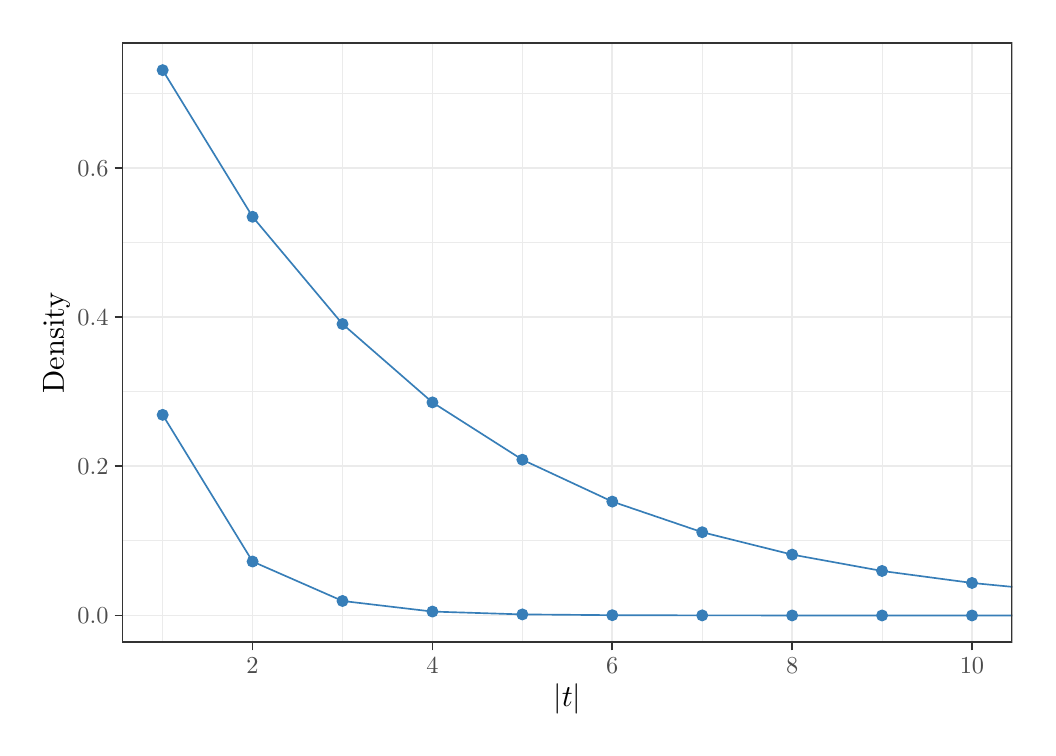
\begin{tikzpicture}[x=1pt,y=1pt]
\definecolor{fillColor}{RGB}{255,255,255}
\path[use as bounding box,fill=fillColor,fill opacity=0.00] (0,0) rectangle (361.35,252.94);
\begin{scope}
\path[clip] (  0.00,  0.00) rectangle (361.35,252.94);
\definecolor{drawColor}{RGB}{255,255,255}
\definecolor{fillColor}{RGB}{255,255,255}

\path[draw=drawColor,line width= 0.6pt,line join=round,line cap=round,fill=fillColor] (  0.00,  0.00) rectangle (361.35,252.94);
\end{scope}
\begin{scope}
\path[clip] ( 34.16, 30.69) rectangle (355.85,247.45);
\definecolor{fillColor}{RGB}{255,255,255}

\path[fill=fillColor] ( 34.16, 30.69) rectangle (355.85,247.45);
\definecolor{drawColor}{gray}{0.92}

\path[draw=drawColor,line width= 0.3pt,line join=round] ( 34.16, 67.49) --
	(355.85, 67.49);

\path[draw=drawColor,line width= 0.3pt,line join=round] ( 34.16,121.40) --
	(355.85,121.40);

\path[draw=drawColor,line width= 0.3pt,line join=round] ( 34.16,175.31) --
	(355.85,175.31);

\path[draw=drawColor,line width= 0.3pt,line join=round] ( 34.16,229.22) --
	(355.85,229.22);

\path[draw=drawColor,line width= 0.3pt,line join=round] ( 48.78, 30.69) --
	( 48.78,247.45);

\path[draw=drawColor,line width= 0.3pt,line join=round] (113.77, 30.69) --
	(113.77,247.45);

\path[draw=drawColor,line width= 0.3pt,line join=round] (178.76, 30.69) --
	(178.76,247.45);

\path[draw=drawColor,line width= 0.3pt,line join=round] (243.74, 30.69) --
	(243.74,247.45);

\path[draw=drawColor,line width= 0.3pt,line join=round] (308.73, 30.69) --
	(308.73,247.45);

\path[draw=drawColor,line width= 0.6pt,line join=round] ( 34.16, 40.54) --
	(355.85, 40.54);

\path[draw=drawColor,line width= 0.6pt,line join=round] ( 34.16, 94.45) --
	(355.85, 94.45);

\path[draw=drawColor,line width= 0.6pt,line join=round] ( 34.16,148.36) --
	(355.85,148.36);

\path[draw=drawColor,line width= 0.6pt,line join=round] ( 34.16,202.27) --
	(355.85,202.27);

\path[draw=drawColor,line width= 0.6pt,line join=round] ( 81.27, 30.69) --
	( 81.27,247.45);

\path[draw=drawColor,line width= 0.6pt,line join=round] (146.26, 30.69) --
	(146.26,247.45);

\path[draw=drawColor,line width= 0.6pt,line join=round] (211.25, 30.69) --
	(211.25,247.45);

\path[draw=drawColor,line width= 0.6pt,line join=round] (276.24, 30.69) --
	(276.24,247.45);

\path[draw=drawColor,line width= 0.6pt,line join=round] (341.23, 30.69) --
	(341.23,247.45);
\definecolor{drawColor}{RGB}{55,126,184}

\path[draw=drawColor,line width= 0.6pt,line join=round] ( 48.78,113.03) --
	( 81.27, 60.03) --
	(113.77, 45.78) --
	(146.26, 41.95) --
	(178.76, 40.92) --
	(211.25, 40.64) --
	(243.74, 40.57) --
	(276.24, 40.55) --
	(308.73, 40.54) --
	(341.23, 40.54) --
	(355.85, 40.54);

\path[draw=drawColor,line width= 0.6pt,line join=round] ( 48.78,237.59) --
	( 81.27,184.60) --
	(113.77,145.85) --
	(146.26,117.53) --
	(178.76, 96.82) --
	(211.25, 81.69) --
	(243.74, 70.62) --
	(276.24, 62.53) --
	(308.73, 56.62) --
	(341.23, 52.29) --
	(355.85, 50.87);
\definecolor{fillColor}{RGB}{55,126,184}

\path[draw=drawColor,line width= 0.4pt,line join=round,line cap=round,fill=fillColor] ( 48.78,113.03) circle (  1.96);

\path[draw=drawColor,line width= 0.4pt,line join=round,line cap=round,fill=fillColor] ( 48.78,237.59) circle (  1.96);

\path[draw=drawColor,line width= 0.4pt,line join=round,line cap=round,fill=fillColor] ( 81.27, 60.03) circle (  1.96);

\path[draw=drawColor,line width= 0.4pt,line join=round,line cap=round,fill=fillColor] ( 81.27,184.60) circle (  1.96);

\path[draw=drawColor,line width= 0.4pt,line join=round,line cap=round,fill=fillColor] (113.77, 45.78) circle (  1.96);

\path[draw=drawColor,line width= 0.4pt,line join=round,line cap=round,fill=fillColor] (113.77,145.85) circle (  1.96);

\path[draw=drawColor,line width= 0.4pt,line join=round,line cap=round,fill=fillColor] (146.26, 41.95) circle (  1.96);

\path[draw=drawColor,line width= 0.4pt,line join=round,line cap=round,fill=fillColor] (146.26,117.53) circle (  1.96);

\path[draw=drawColor,line width= 0.4pt,line join=round,line cap=round,fill=fillColor] (178.76, 40.92) circle (  1.96);

\path[draw=drawColor,line width= 0.4pt,line join=round,line cap=round,fill=fillColor] (178.76, 96.82) circle (  1.96);

\path[draw=drawColor,line width= 0.4pt,line join=round,line cap=round,fill=fillColor] (211.25, 40.64) circle (  1.96);

\path[draw=drawColor,line width= 0.4pt,line join=round,line cap=round,fill=fillColor] (211.25, 81.69) circle (  1.96);

\path[draw=drawColor,line width= 0.4pt,line join=round,line cap=round,fill=fillColor] (243.74, 40.57) circle (  1.96);

\path[draw=drawColor,line width= 0.4pt,line join=round,line cap=round,fill=fillColor] (243.74, 70.62) circle (  1.96);

\path[draw=drawColor,line width= 0.4pt,line join=round,line cap=round,fill=fillColor] (276.24, 40.55) circle (  1.96);

\path[draw=drawColor,line width= 0.4pt,line join=round,line cap=round,fill=fillColor] (276.24, 62.53) circle (  1.96);

\path[draw=drawColor,line width= 0.4pt,line join=round,line cap=round,fill=fillColor] (308.73, 40.54) circle (  1.96);

\path[draw=drawColor,line width= 0.4pt,line join=round,line cap=round,fill=fillColor] (308.73, 56.62) circle (  1.96);

\path[draw=drawColor,line width= 0.4pt,line join=round,line cap=round,fill=fillColor] (341.23, 40.54) circle (  1.96);

\path[draw=drawColor,line width= 0.4pt,line join=round,line cap=round,fill=fillColor] (341.23, 52.29) circle (  1.96);
\definecolor{drawColor}{gray}{0.20}

\path[draw=drawColor,line width= 0.9pt,line join=round,line cap=round] ( 34.16, 30.69) rectangle (355.85,247.45);
\end{scope}
\begin{scope}
\path[clip] (  0.00,  0.00) rectangle (361.35,252.94);
\definecolor{drawColor}{gray}{0.30}

\node[text=drawColor,anchor=base east,inner sep=0pt, outer sep=0pt, scale=  0.88] at ( 29.21, 37.51) {0.0};

\node[text=drawColor,anchor=base east,inner sep=0pt, outer sep=0pt, scale=  0.88] at ( 29.21, 91.42) {0.2};

\node[text=drawColor,anchor=base east,inner sep=0pt, outer sep=0pt, scale=  0.88] at ( 29.21,145.33) {0.4};

\node[text=drawColor,anchor=base east,inner sep=0pt, outer sep=0pt, scale=  0.88] at ( 29.21,199.24) {0.6};
\end{scope}
\begin{scope}
\path[clip] (  0.00,  0.00) rectangle (361.35,252.94);
\definecolor{drawColor}{gray}{0.20}

\path[draw=drawColor,line width= 0.6pt,line join=round] ( 31.41, 40.54) --
	( 34.16, 40.54);

\path[draw=drawColor,line width= 0.6pt,line join=round] ( 31.41, 94.45) --
	( 34.16, 94.45);

\path[draw=drawColor,line width= 0.6pt,line join=round] ( 31.41,148.36) --
	( 34.16,148.36);

\path[draw=drawColor,line width= 0.6pt,line join=round] ( 31.41,202.27) --
	( 34.16,202.27);
\end{scope}
\begin{scope}
\path[clip] (  0.00,  0.00) rectangle (361.35,252.94);
\definecolor{drawColor}{gray}{0.20}

\path[draw=drawColor,line width= 0.6pt,line join=round] ( 81.27, 27.94) --
	( 81.27, 30.69);

\path[draw=drawColor,line width= 0.6pt,line join=round] (146.26, 27.94) --
	(146.26, 30.69);

\path[draw=drawColor,line width= 0.6pt,line join=round] (211.25, 27.94) --
	(211.25, 30.69);

\path[draw=drawColor,line width= 0.6pt,line join=round] (276.24, 27.94) --
	(276.24, 30.69);

\path[draw=drawColor,line width= 0.6pt,line join=round] (341.23, 27.94) --
	(341.23, 30.69);
\end{scope}
\begin{scope}
\path[clip] (  0.00,  0.00) rectangle (361.35,252.94);
\definecolor{drawColor}{gray}{0.30}

\node[text=drawColor,anchor=base,inner sep=0pt, outer sep=0pt, scale=  0.88] at ( 81.27, 19.68) {2};

\node[text=drawColor,anchor=base,inner sep=0pt, outer sep=0pt, scale=  0.88] at (146.26, 19.68) {4};

\node[text=drawColor,anchor=base,inner sep=0pt, outer sep=0pt, scale=  0.88] at (211.25, 19.68) {6};

\node[text=drawColor,anchor=base,inner sep=0pt, outer sep=0pt, scale=  0.88] at (276.24, 19.68) {8};

\node[text=drawColor,anchor=base,inner sep=0pt, outer sep=0pt, scale=  0.88] at (341.23, 19.68) {10};
\end{scope}
\begin{scope}
\path[clip] (  0.00,  0.00) rectangle (361.35,252.94);
\definecolor{drawColor}{RGB}{0,0,0}

\node[text=drawColor,anchor=base,inner sep=0pt, outer sep=0pt, scale=  1.10] at (195.00,  7.64) {$|t|$};
\end{scope}
\begin{scope}
\path[clip] (  0.00,  0.00) rectangle (361.35,252.94);
\definecolor{drawColor}{RGB}{0,0,0}

\node[text=drawColor,rotate= 90.00,anchor=base,inner sep=0pt, outer sep=0pt, scale=  1.10] at ( 13.08,139.07) {Density};
\end{scope}
\end{tikzpicture}
